\documentclass[11pt,a4paper]{article}
\usepackage[utf8]{inputenc}
\usepackage[T1]{fontenc}
\usepackage{lmodern}
\usepackage{geometry}
\usepackage{graphicx}
\usepackage{enumitem}
\usepackage{xcolor}
\usepackage{fancyhdr}
\usepackage{titlesec}
\usepackage{tikz}
\usetikzlibrary{shapes.geometric, arrows.meta, positioning, fit, backgrounds}

% Commande pour les numéros encerclés dans le texte
\newcommand{\circled}[1]{\tikz[baseline=(char.base)]{\node[shape=circle,draw,inner sep=2pt,fill=white,font=\bfseries\small] (char) {#1};}}

% Symboles case à cocher (Unicode)
\newcommand{\checksymbol}{\textcolor{black}{\textbf{☑}}}
\newcommand{\unchecksymbol}{\textcolor{black}{\textbf{☐}}}

\geometry{margin=2.5cm}
\pagestyle{fancy}
\fancyhf{}
\fancyhead[L]{Internship Report — IFC Analyzer Platform}
\fancyhead[R]{\thepage}
\renewcommand{\headrulewidth}{0.4pt}

\definecolor{usercolor}{RGB}{59,130,246}
\definecolor{systemcolor}{RGB}{16,185,129}
\definecolor{dbcolor}{RGB}{139,92,246}
\definecolor{processcolor}{RGB}{245,158,11}

\titleformat{\section}{\Large\bfseries\color{usercolor}}{\thesection}{1em}{}
\titleformat{\subsection}{\large\bfseries\color{systemcolor}}{\thesubsection}{1em}{}

\begin{document}

% ============================================================
% TITLE PAGE
% ============================================================
\begin{titlepage}
\centering
\vspace*{2cm}
{\Huge\bfseries Internship Report\\[0.5cm]
\Large IFC Analyzer — BIM-Based Component Management Platform\\[2cm]}
{\large Zineddine NIRAK\\[0.3cm]
May 2026\\[3cm]}
\vfill
\end{titlepage}

% ============================================================
% TABLE OF CONTENTS
% ============================================================
\tableofcontents
\newpage

% ============================================================
\section{Introduction}
% ============================================================

The construction industry generates a significant amount of waste and consumes a large quantity of raw materials every year. In recent years, sustainable construction and circular economy principles have become major priorities in the Architecture, Engineering, and Construction (AEC) sector.

Building Information Modeling (BIM) offers new opportunities to improve building lifecycle management by providing intelligent digital representations of buildings and their components. However, many existing BIM workflows focus mainly on design and construction phases, while the reuse and recovery of building components remain insufficiently explored.

This project proposes a BIM-based platform designed to support building component extraction, tracking, visualization, and reuse management using IFC models. The platform aims to facilitate the identification of reusable elements and assist professionals during selective deconstruction and material recovery processes.

The system integrates several functionalities, including:
\begin{itemize}
    \item automatic extraction of building components from IFC files,
    \item tracking and classification of reusable materials,
    \item interactive 3D visualization of building elements,
    \item and semi-automatic generation of PEMD-related information for reusable components.
\end{itemize}

The objective of this work is to demonstrate how BIM technologies can contribute to more sustainable construction practices and improve material circularity in the construction sector.

% ============================================================
\section{Problem Statement}
% ============================================================

The construction industry is one of the largest consumers of raw materials and one of the main contributors to global waste generation and carbon emissions. In this context, the transition toward a circular economy has become a major priority, aiming to extend the lifecycle of building materials through reuse, recycling, and recovery strategies instead of disposal.

Building Information Modeling (BIM) has significantly improved the way buildings are designed, constructed, and managed. However, its potential in supporting circular economy practices, particularly during renovation and deconstruction phases, remains limited. Most BIM applications are still focused on the design and construction stages, with insufficient support for end-of-life decision-making.

A key challenge lies in the lack of effective methods to exploit the rich information contained in IFC models for material recovery purposes. Although IFC files store detailed geometric and semantic data about building components, this information is often not structured or accessible in a way that supports decision-making for reuse, recycling, or dismantling strategies.

Furthermore, current workflows do not provide sufficient tools for classifying, tracking, and managing building components during deconstruction processes. This results in poor visibility of material flows, limited traceability of components, and reduced ability to evaluate their recovery potential. As a consequence, valuable materials are often discarded instead of being reintegrated into new construction cycles.

Another limitation is the absence of integrated digital solutions capable of linking BIM data with circular economy requirements such as PEMD reporting, material inventories, and selective deconstruction planning. This gap prevents a fully data-driven approach to sustainable building lifecycle management.

Therefore, there is a clear need for a BIM-based system that supports structured extraction, organization, and visualization of building components in order to enable efficient material recovery and to promote circular economy principles in the construction sector.

% ============================================================
\section{Objectives}
% ============================================================

The main objective of this project is to develop a BIM-based platform capable of assisting professionals in the identification, tracking, and management of building components during deconstruction, renovation, and end-of-life processes.

The platform is designed to improve material recovery workflows by combining Building Information Modeling (BIM) technologies with interactive visualization and component management functionalities.

The project focuses on the following objectives:

\begin{itemize}
    \item Automatically extract building elements and their associated information from IFC models;
    \item Organize and classify building components according to their type, material, and IFC properties;
    \item Provide an interactive 3D visualization environment for exploring building elements and their geometric and semantic information;
    \item Enable tracking of building components throughout different stages of the deconstruction and renovation process;
    \item Assist in the generation of PEMD-related information based on extracted building components;
    \item Contribute to circular economy practices in the construction sector by improving material understanding, traceability, and waste reduction.
\end{itemize}

% ============================================================
\section{Proposed Platform}
% ============================================================

To address the challenges discussed in the previous section, a BIM-based platform was developed to support the management of building components during renovation, deconstruction, and material recovery processes. The platform aims to facilitate the exploitation of information contained in IFC models and transform it into actionable data for circular economy applications.

The proposed platform serves as a centralized environment where building information can be extracted, organized, visualized, and managed throughout different stages of a building's lifecycle. By leveraging BIM data, the system provides users with a better understanding of building components and their associated characteristics, including geometry, materials, quantities, and semantic properties.

The platform is designed around several core functionalities. First, it enables the automatic extraction of building elements and their associated information from IFC files. The extracted data is then structured and organized to create a comprehensive inventory of building components.

Second, the platform provides interactive 3D visualization capabilities, allowing users to explore BIM models and inspect individual elements together with their associated information. This visualization layer facilitates the analysis and interpretation of building data.

Third, the system supports component tracking and status management. Building elements can be monitored throughout renovation and deconstruction processes, enabling stakeholders to maintain updated information regarding their condition and recovery strategy.

Finally, the platform contributes to the preparation of PEMD-related information by providing structured access to building component data and material inventories. This functionality supports decision-making processes related to material recovery and circular economy practices.

Overall, the proposed platform aims to bridge the gap between BIM data and circular economy requirements by providing an integrated solution for component extraction, visualization, tracking, and management.

% ============================================================
\section{System Workflow (Detailed)}
% ============================================================
\label{sec:workflow}

This section describes in detail the complete system workflow, covering the authentication module, the extraction module, the tracking module, and the 3D visualization module.

% --------------------------------------------------------
\subsection{Authentication Module}
% --------------------------------------------------------

\subsubsection{Registration Flow}

\begin{enumerate}[leftmargin=*]
    \item \textbf{User Action:} Navigate to \texttt{/login} page.
    \item \textbf{User Action:} Fill email and password (minimum 8 characters).
    \item \textbf{User Action:} Click \textbf{``Create Account''} button.
    \item \textbf{System Process:} Frontend sends \texttt{POST /api/auth/register} with credentials.
    \item \textbf{Backend Validation:} 
        \begin{itemize}
            \item Check if email already exists (unique constraint).
            \item Hash password using bcrypt.
            \item Store user in SQLite auth database with role \texttt{user}.
        \end{itemize}
    \item \textbf{System Response:} Return user data (id, email, role).
    \item \textbf{Frontend Action:} Auto-login after registration.
    \item \textbf{Token Generation:} Backend creates JWT token (expires in 60 min).
    \item \textbf{Storage:} Token saved in browser \texttt{localStorage}.
    \item \textbf{Redirect:} User redirected to home page \texttt{/}.
\end{enumerate}

\subsubsection{Login Flow}

\begin{enumerate}[leftmargin=*]
    \item \textbf{User Action:} Enter email and password on \texttt{/login}.
    \item \textbf{User Action:} Click \textbf{``Login''} button.
    \item \textbf{System Process:} Frontend sends \texttt{POST /api/auth/login}.
    \item \textbf{Backend Validation:}
        \begin{itemize}
            \item Verify email exists.
            \item Compare password hash with bcrypt.
        \end{itemize}
    \item \textbf{Token Generation:} Create JWT token with user id and role.
    \item \textbf{Storage:} Token saved in \texttt{localStorage}.
    \item \textbf{Auth Wrapper:} All subsequent API calls include \texttt{Authorization: Bearer <token>} header.
    \item \textbf{Session Management:} On 401 response, clear token and redirect to login.
\end{enumerate}

\subsubsection{Role-Based Access Control}

\begin{itemize}
    \item \textbf{User Role:} Can create projects, extract IFC, track components, export reports.
    \item \textbf{Admin Role:} Can list all users, change user roles.
    \item \textbf{Public Routes:} Health check, login, register, public component details (QR codes).
\end{itemize}

% --------------------------------------------------------
\subsection{Extraction Module}
% --------------------------------------------------------

\subsubsection{IFC Upload and Analysis}

The extraction process begins on the ``IFC Data Extraction'' page (Figure~\ref{fig:extraction-upload}). The user uploads an IFC file through the drag-and-drop interface or by using the file selector.

\begin{figure}[h]
    \centering
    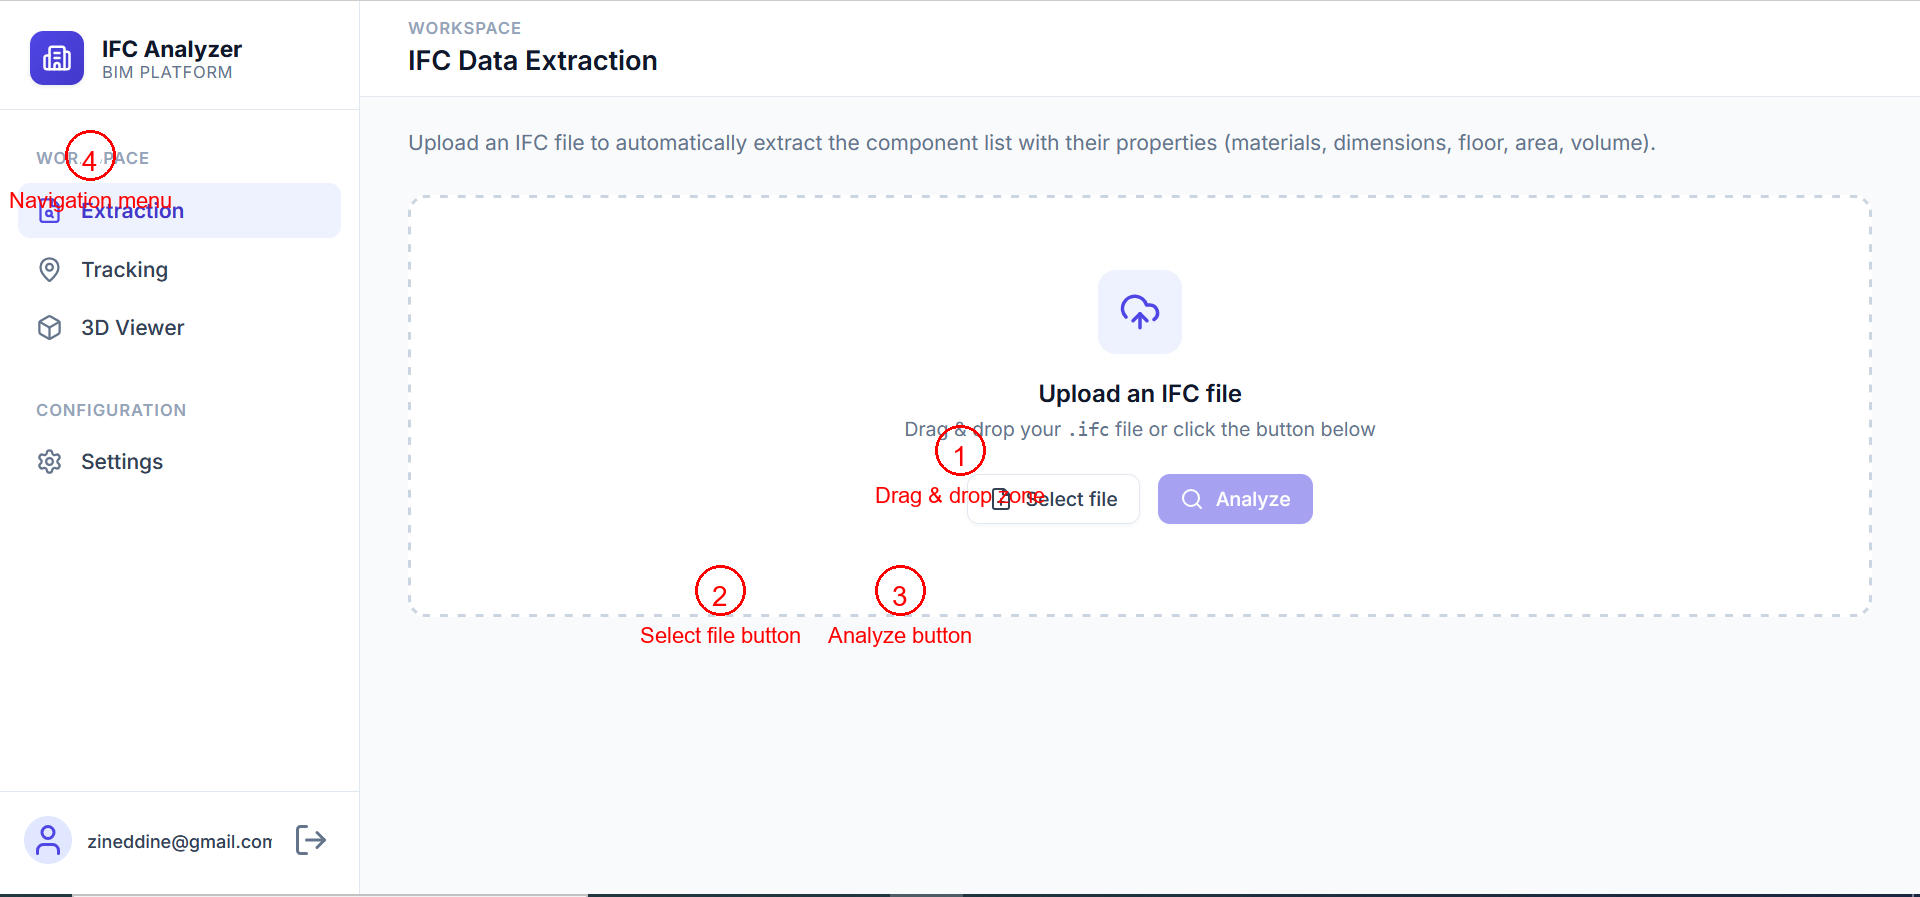
\includegraphics[width=0.95\textwidth]{screenshots/extraction-upload-annotated.png}
    \caption{IFC Upload Interface — Step 1: File Selection and Analysis}
    \label{fig:extraction-upload}
\end{figure}

\noindent\textbf{Interface elements (Figure~\ref{fig:extraction-upload}):}

\begin{enumerate}[leftmargin=*]
    \item[\circled{1}] \textbf{Drag \& Drop Zone:} Central area where the user can drag and drop an \texttt{.ifc} file. The dashed border indicates the drop target.
    \item[\circled{2}] \textbf{Select File Button:} Opens the system file picker to browse for an IFC file. Only files with the \texttt{.ifc} extension are accepted.
    \item[\circled{3}] \textbf{Analyze Button:} Once a file is selected, this button triggers the upload and processing. It sends a \texttt{POST /api/upload} request with the file via multipart/form-data.
    \item[\circled{4}] \textbf{Navigation Menu:} Left sidebar providing access to the three main modules: Extraction, Tracking, and 3D Viewer.
\end{enumerate}

\vspace{0.5cm}

\noindent\textbf{Backend Processing:}

Once the file is uploaded, the backend performs the following operations:

\begin{enumerate}[leftmargin=*]
    \item \textbf{File Validation:} Check file extension (must be \texttt{.ifc}).
    \item \textbf{Temporary Storage:} Save file to disk for processing.
    \item \textbf{IFC Parsing:} Parse the IFC model using \texttt{ifcopenshell}.
    \item \textbf{Element Extraction:} Extract building elements including:
        \begin{itemize}
            \item Walls, Windows, Doors, Slabs, Stairs, Curtain Walls.
            \item Properties: Height, Length, Thickness, Volume, Material, Floor/Level.
        \end{itemize}
    \item \textbf{Dimension Conversion:} Convert dimensions from mm to meters (if value > 10).
    \item \textbf{Sustainability Scoring:} Calculate Recyclability (0--1) and Reusability (0--1) based on material type.
    \item \textbf{Data Enrichment:} Apply business rules (e.g., concrete = low reusability, steel = high recyclability).
\end{enumerate}

\subsubsection{Extraction Results Display}

After analysis, the platform displays the extracted data in a structured interface (Figure~\ref{fig:extraction-results}).

\begin{figure}[h]
    \centering
    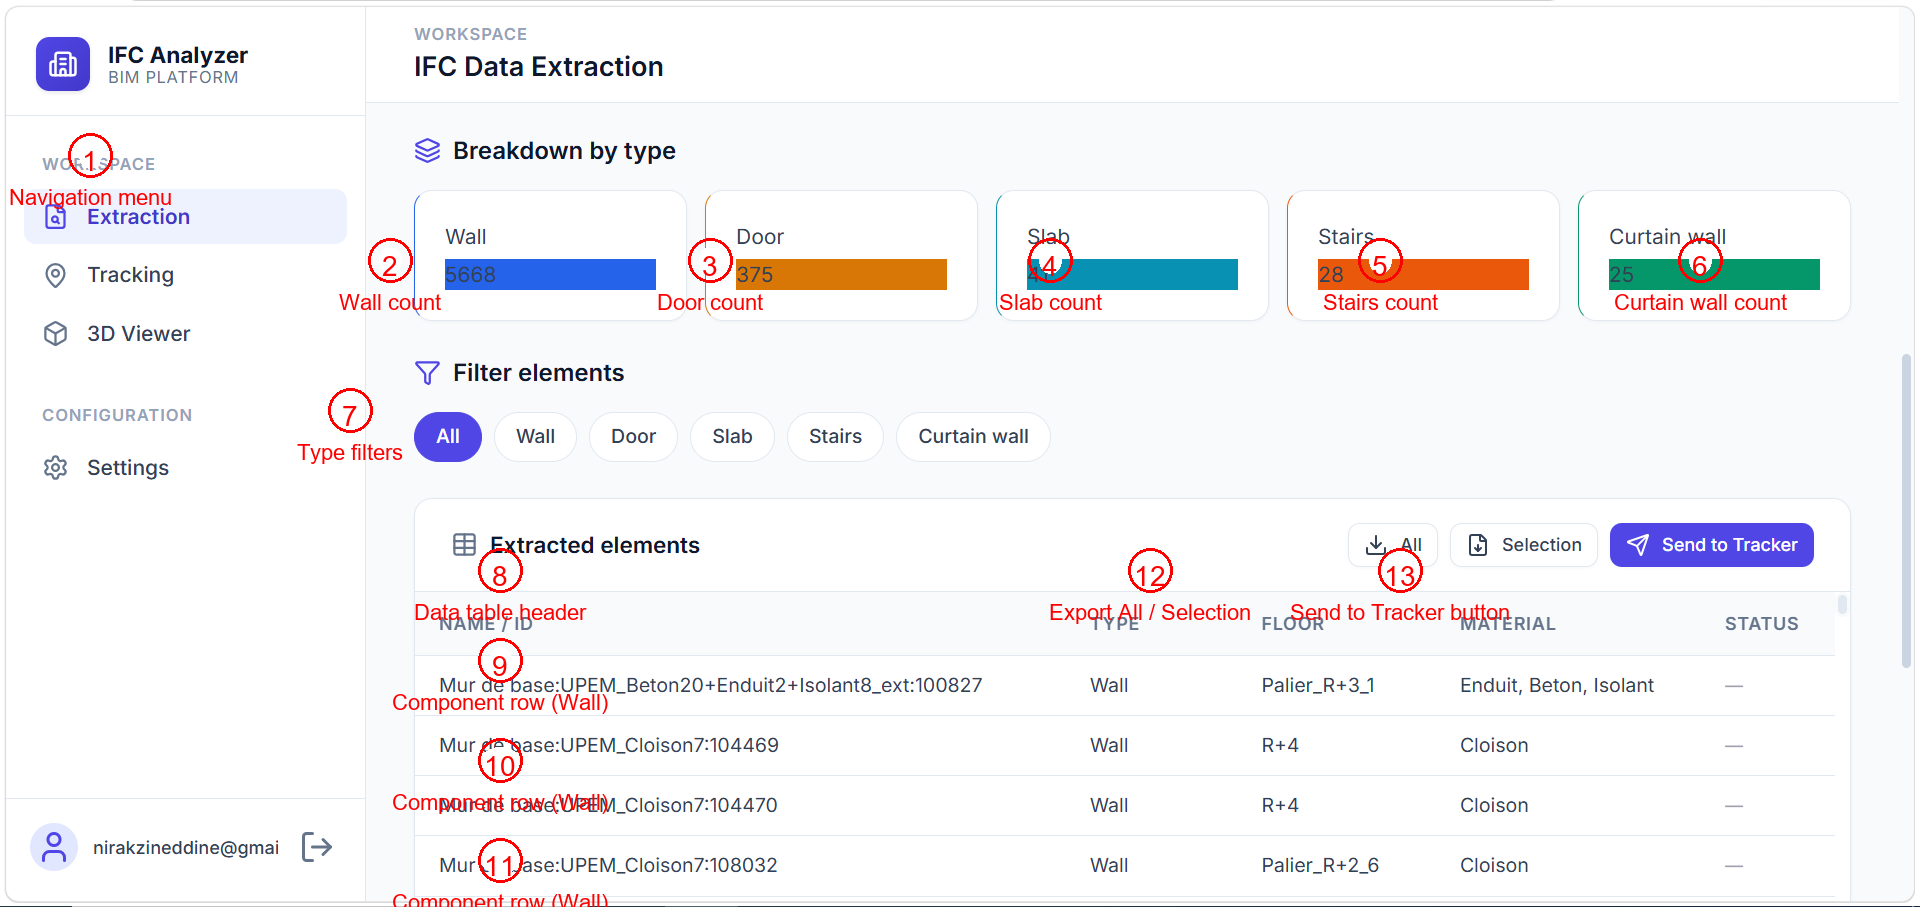
\includegraphics[width=0.95\textwidth]{screenshots/extraction-results-annotated.png}
    \caption{Extraction Results — Component List with Summary and Filters}
    \label{fig:extraction-results}
\end{figure}

\noindent\textbf{Interface elements (Figure~\ref{fig:extraction-results}):}

\begin{enumerate}[leftmargin=*]
    \item[\circled{1}] \textbf{Navigation Menu:} Same sidebar as in Figure~\ref{fig:extraction-upload}, showing the active module (Extraction).
    \item[\circled{2}--\circled{6}] \textbf{Summary Cards (Breakdown by Type):} Horizontal cards showing the count of each element type. The bar width is proportional to the count:
        \begin{itemize}
            \item \circled{2} Wall: 5668 elements (largest category)
            \item \circled{3} Door: 375 elements
            \item \circled{4} Slab: 41 elements
            \item \circled{5} Stairs: 28 elements
            \item \circled{6} Curtain wall: 25 elements
        \end{itemize}
    \item[\circled{7}] \textbf{Type Filters:} Clickable filter buttons to show only elements of a specific type (e.g., ``All'', ``Wall'', ``Door'', ``Slab'', ``Stairs'', ``Curtain wall'').
    \item[\circled{8}] \textbf{Data Table Header:} Columns showing: NAME/ID, TYPE, FLOOR, MATERIAL, STATUS.
    \item[\circled{9}--\circled{11}] \textbf{Data Rows:} Each row represents one IFC component with:
        \begin{itemize}
            \item \textbf{NAME/ID:} The IFC element identifier (e.g., ``Mur de base:UPEM\_Beton20+Enduit2+Isolant8\_ext:100827'')
            \item \textbf{TYPE:} Mapped type (e.g., ``Wall'', ``Door'')
            \item \textbf{FLOOR:} Building level (e.g., ``Palier\_R+3\_1'', ``R+4'')
            \item \textbf{MATERIAL:} Material composition (e.g., ``Enduit, Beton, Isolant'', ``Cloison'')
            \item \textbf{STATUS:} Tracker status if available, otherwise ``---''
        \end{itemize}
    \item[\circled{12}] \textbf{Export Buttons:} ``All'' (export all elements) and ``Selection'' (export filtered elements) in CSV or PDF format.
    \item[\circled{13}] \textbf{Send to Tracker:} Primary action button that sends all extracted components to the Tracking module for lifecycle management.
\end{enumerate}

\vspace{0.5cm}

\noindent\textbf{Local Storage:} Results are cached in the browser's IndexedDB for offline viewing and persistence across page navigations.

\subsubsection{Status Synchronization from Tracker}

\begin{enumerate}[leftmargin=*]
    \item \textbf{Background Process:} After extraction, frontend calls \texttt{POST /api/public/statuses}.
    \item \textbf{System Process:} Backend queries tracker database for component statuses.
    \item \textbf{Data Merge:} If component exists in tracker, show its current status (e.g., ``dismantled'', ``stored'').
    \item \textbf{Default Status:} If not tracked, show ``in\_building''.
    \item \textbf{UI Update:} Status badges dynamically added to table rows.
\end{enumerate}

\subsubsection{Send to Tracker}

\begin{enumerate}[leftmargin=*]
    \item \textbf{User Action:} Click \textbf{``Send to Tracker''} button after extraction.
    \item \textbf{User Action:} Enter project name (or accept default with date).
    \item \textbf{System Process:} Frontend sends \texttt{POST /api/tracker/import} with:
        \begin{itemize}
            \item Array of components (ID, type, material, dimensions, status).
            \item Project name.
        \end{itemize}
    \item \textbf{Backend Processing:}
        \begin{itemize}
            \item Create new project in SQLite tracker database with current \texttt{user\_id}.
            \item Import components with status ``in\_building''.
            \item If component ID already exists in another project, suffix with \texttt{\_\_p\{project\_id\}}.
            \item Add initial status history entry: ``Import initial IFC''.
        \end{itemize}
    \item \textbf{System Response:} Return project ID, name, and count of imported components.
    \item \textbf{Frontend Action:} Show success message and offer to navigate to Tracker.
\end{enumerate}

\subsubsection{PEMD Export (CERFA Tableau 1)}

The PEMD (Produits, Équipements et Matériaux du Démantèlement) report is a regulatory requirement in France for documenting potentially reusable building materials. The platform automates the extraction of this information while allowing manual validation and editing before export.

\paragraph{Preparing Components for PEMD Export}

Before generating the PEMD report, the user must first identify and mark the components that are potentially reusable. This workflow is performed directly from the Tracking module (Figure~\ref{fig:tracking-pemd-prep}).

\begin{figure}[h]
    \centering
    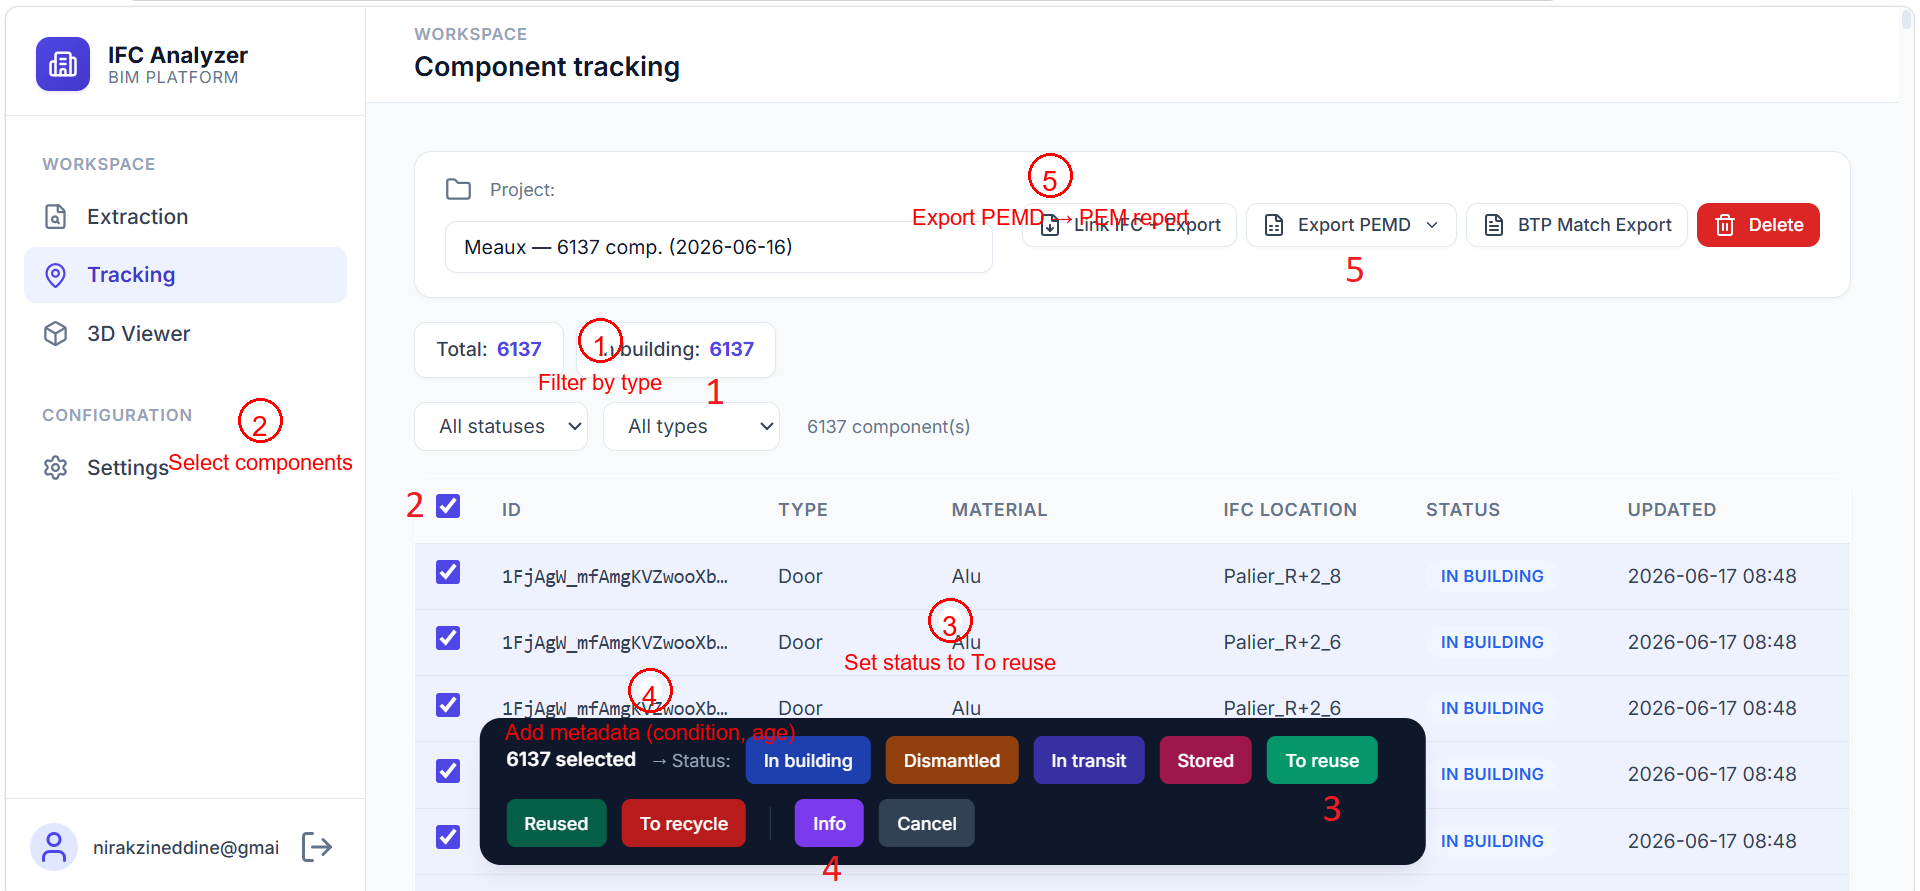
\includegraphics[width=0.95\textwidth]{screenshots/tracking-pemd-prep-annotated.png}
    \caption{Preparing Components for PEMD Export — Tracking Module Workflow}
    \label{fig:tracking-pemd-prep}
\end{figure}

\noindent\textbf{Workflow steps (Figure~\ref{fig:tracking-pemd-prep}):}

\begin{enumerate}[leftmargin=*]
    \item[\circled{1}] \textbf{Filter by Type:} The user can filter the component list by type (e.g., only Doors, Slabs, Walls) using the ``All types'' dropdown. This helps focus on specific categories of reusable materials.
    
    \item[\circled{2}] \textbf{Select Components:} The user selects one or more components using the checkboxes in the table. The header checkbox allows bulk selection of all visible components. Individual checkboxes allow precise selection.
    
    \item[\circled{3}] \textbf{Set Status to ``To reuse'':} Once components are selected, a bulk action bar appears at the bottom. The user clicks \textbf{``To reuse''} (green button). This status is essential because the PEMD report only includes components marked as ``à réutiliser'' (to reuse). The system records this status change in the component history.
    
    \item[\circled{4}] \textbf{Add Metadata (Condition \& Age):} The user clicks the \textbf{``Info''} button (purple button) in the bulk action bar. A modal opens allowing the user to set:
        \begin{itemize}
            \item \textbf{Condition:} Neuf (New), Bon (Good), Moyen (Fair), or Mauvais (Poor).
            \item \textbf{Estimated Age:} Under 2 years, 2--10 years, 10--50 years, or Over 50 years.
        \end{itemize}
        This metadata is stored in the tracker database and will be pre-filled in the PEMD report.
    
    \item[\circled{5}] \textbf{Export PEMD:} After marking components as ``To reuse'' and adding metadata, the user clicks the \textbf{``Export PEMD''} dropdown button in the toolbar and selects \textbf{``PEM report''}. This opens the interactive PEMD preview modal where the user can review and edit the data before final export.
\end{enumerate}

\vspace{0.3cm}

\noindent\textbf{Key Design Point:} Only components with status ``à réutiliser'' are included in the PEMD report. This ensures the report exclusively contains materials that have been identified as potentially reusable, avoiding clutter from components that are still in building, already recycled, or destined for disposal.

\paragraph{Grouped Data Generation}

The system groups components by (type, material, dimensions) to produce CERFA-compliant rows:

\begin{enumerate}[leftmargin=*]
    \item \textbf{Backend Processing:} When the user opens the PEMD report, the backend queries all components with status ``à réutiliser'' (to reuse) from the tracker database.
    \item \textbf{IFC Enrichment:} For each component, the system retrieves stored dimensions (height, length, thickness) from the database. If the original IFC file was uploaded, it also parses the IFC model to extract additional geometric data (net volume, net area).
    \item \textbf{Grouping:} Components are grouped by (type, material, dimensions\_key). This ensures that, for example, 20 aluminum windows of dimension X and 30 aluminum windows of dimension Y appear as two separate lines.
    \item \textbf{Quantity Calculation:} Quantities are computed according to the CERFA unit convention:
        \begin{itemize}
            \item Walls, slabs, curtain walls $\rightarrow$ m\textsuperscript{2} (sum of net area).
            \item Windows, doors, stairs $\rightarrow$ U (unit count).
            \item Linear elements $\rightarrow$ ml (sum of length).
            \item Volumetric elements $\rightarrow$ m\textsuperscript{3} (sum of net volume).
        \end{itemize}
    \item \textbf{Description Auto-fill:} The description field is auto-generated as ``Type in material — dimensions''.
\end{enumerate}

\paragraph{Interactive Preview and Edit Modal}

Before exporting, the user can preview and edit the PEMD data in an interactive modal (Figure~\ref{fig:pemd-modal}). This modal displays all components marked as ``\`{a} r\'{e}utiliser'' in a CERFA-compliant table.

\begin{figure}[h]
    \centering
    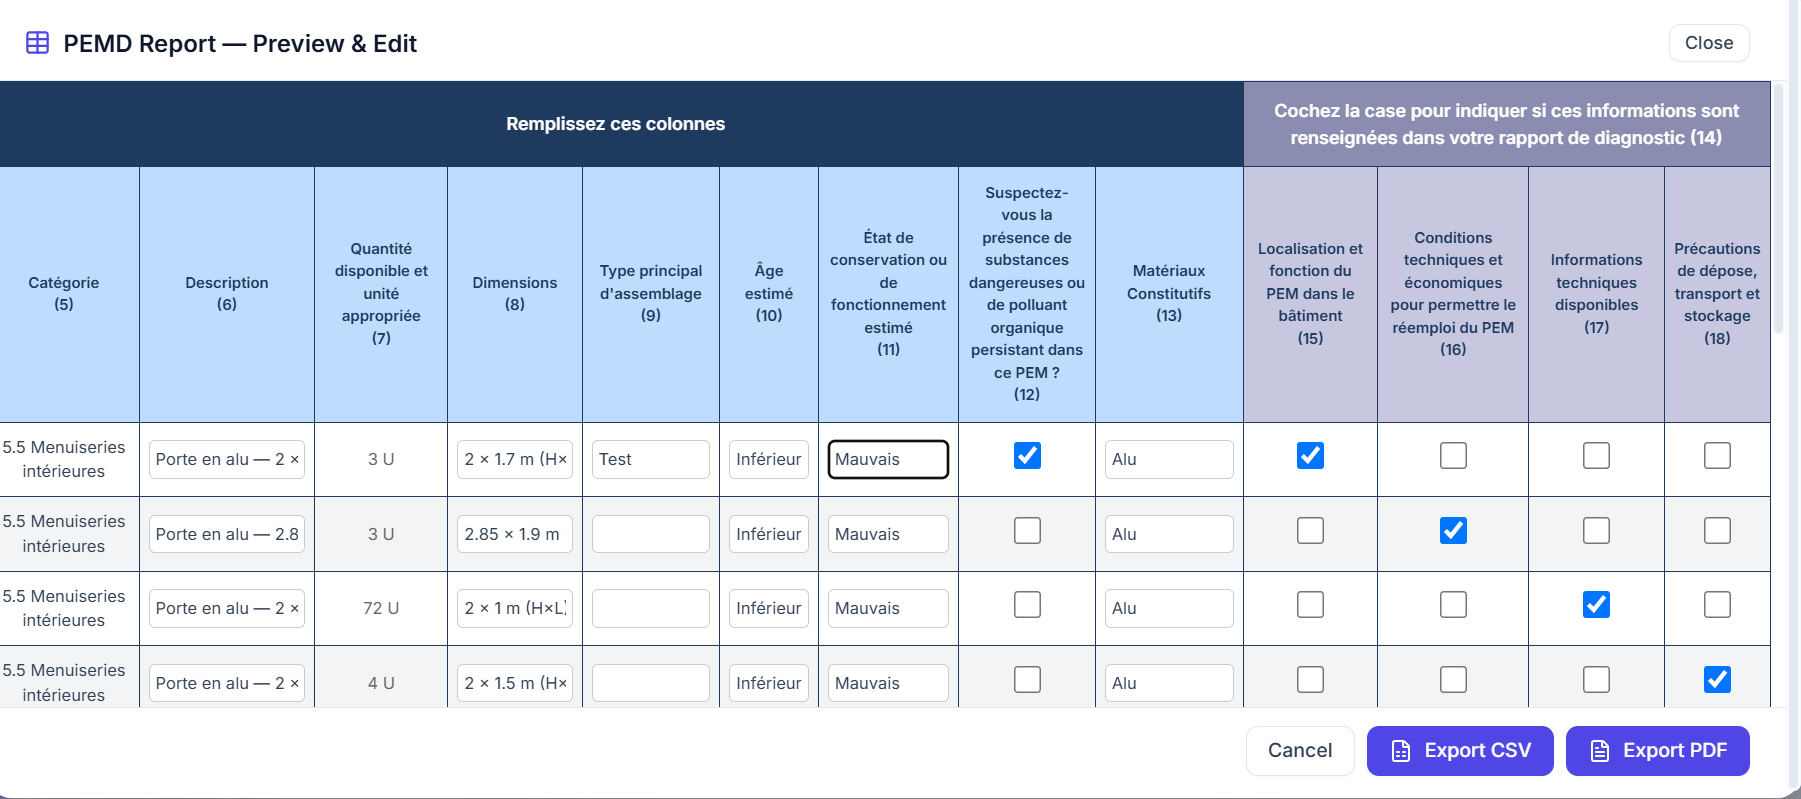
\includegraphics[width=0.95\textwidth]{screenshots/pemd-modal.png}
    \caption{PEMD Report Preview and Edit Modal (CERFA Tableau 1)}
    \label{fig:pemd-modal}
\end{figure}

\noindent\textbf{Component Grouping Logic}

Components are not listed individually. Instead, the system groups them by a composite key: \textbf{(type, material, dimensions)}. This grouping is essential for the PEMD report because it mirrors how materials are actually inventoried on a construction site. For example:

\begin{itemize}
    \item 20 aluminum doors of size $2.0 \times 1.7$~m will appear as a single line with quantity ``20~U''.
    \item 30 aluminum doors of size $2.85 \times 1.9$~m will appear as a \textit{separate} line.
    \item 72 aluminum doors of size $2.0 \times 1.0$~m will form a third distinct group.
\end{itemize}

This differentiation by dimensions is crucial: merging different sizes into a single line would make the report unusable for deconstruction planning. The user can verify and, if necessary, correct the dimensions in the editable fields before export.

\noindent\textbf{Editable Fields and User Modifications}

The modal allows the user to review and modify every field before generating the final report:

\begin{itemize}
    \item \textbf{Category (5):} Automatically mapped from the component type to the official CERFA nomenclature. For example, ``Porte'' (Door) is mapped to ``5.5 Menuiseries int\'{e}rieures''. This mapping uses the standardized PEMD classification table and cannot be edited by the user, ensuring regulatory compliance.
    
    \item \textbf{Description (6):} Pre-filled with the component type, material, and dimensions (e.g., ``Porte en alu --- 2 $\times$ 1.7 m''). The user can edit this text to add more details or correct the auto-generated description.
    
    \item \textbf{Quantity (7):} Automatically computed based on the component type and available geometric data. The unit follows the CERFA convention:
        \begin{itemize}
            \item Doors, windows, stairs $\rightarrow$ count in units (U), e.g., ``3~U''.
            \item Walls, slabs, curtain walls $\rightarrow$ area in m\textsuperscript{2}.
            \item Linear elements $\rightarrow$ length in ml.
            \item Volumetric elements $\rightarrow$ volume in m\textsuperscript{3}.
        \end{itemize}
        The quantity field is read-only because it is derived from the grouped component count.
    
    \item \textbf{Dimensions (8):} Pre-filled from IFC data or tracker storage (e.g., ``2 $\times$ 1.7 m (H$\times$L)''). If the IFC extraction was incomplete or approximate, the user can manually enter the correct dimensions.
    
    \item \textbf{Assembly Type (9):} Left empty by default because it cannot be reliably inferred from the IFC model. The user must fill this field manually (e.g., ``M\'{e}canique'', ``Chimique permanent'').
    
    \item \textbf{Age (10):} Pre-filled from tracker metadata if the user previously set an estimated age via the ``Info'' bulk action.
    
    \item \textbf{Condition (11):} Pre-filled from tracker metadata (Neuf, Bon, Moyen, Mauvais). The user can override this value directly in the modal.
    
    \item \textbf{Materials (13):} Pre-filled with the component material (e.g., ``Alu'').
\end{itemize}

\noindent\textbf{Checkboxes for CERFA Compliance (Columns 12, 15--18)}

The right section of the table contains checkboxes that indicate whether specific information is present in the diagnostic report, exactly as required by the CERFA form:

\begin{itemize}
    \item \textbf{Column (12):} Suspect hazardous substances or persistent organic pollutants.
    \item \textbf{Column (15):} Location and function of the PEM in the building.
    \item \textbf{Column (16):} Technical and economic conditions enabling reuse.
    \item \textbf{Column (17):} Technical information available.
    \item \textbf{Column (18):} Precautions for removal, transport, and storage.
\end{itemize}

By default, all checkboxes are unchecked (empty). The user must actively check the boxes that apply to each component group. This design follows the strict rule of \textbf{no invented data}: the platform never guesses whether a material contains hazardous substances or whether reuse conditions are met.

\noindent\textbf{Visual Style}

The table header replicates the official CERFA color scheme: a blue section (\#1e3a5f) for the left columns labeled ``Remplissez ces colonnes'' and a purple section (\#8b8db0) for the right columns labeled ``Cochez la case pour indiquer si ces informations sont renseign\'{e}es dans votre rapport de diagnostic''. This visual separation helps users quickly identify which fields require manual input versus which fields require verification.

\paragraph{Export Formats}

After editing, the user can export the PEMD report in two formats:

\begin{enumerate}[leftmargin=*]
    \item \textbf{Export CSV:}
        \begin{itemize}
            \item UTF-8 with BOM, semicolon-separated (French Excel standard).
            \item Headers: (5) Catégorie, (6) Description, (7) Quantité, (8) Dimensions, (9) Assemblage, (10) Âge, (11) État, (12) Dangereuses, (13) Matériaux, (15) Localisation, (16) Conditions, (17) Infos techniques, (18) Précautions.
            \item Checkbox columns: ``Oui'' if checked, empty if unchecked.
        \end{itemize}
    \item \textbf{Export PDF:}
        \begin{itemize}
            \item Landscape A4 with the exact CERFA table layout.
            \item Uses TTF fonts (DejaVu Sans or Arial) to render Unicode checkbox symbols: \texttt{☑} for checked, \texttt{☐} for unchecked.
            \item Color-coded header: blue for left columns, purple for right columns.
            \item Alternating row colors (white / light gray) for readability.
        \end{itemize}
\end{enumerate}

\begin{figure}[h]
    \centering
    \includegraphics[width=0.95\textwidth]{screenshots/pemd-pdf.png}
    \caption{Exported PEMD PDF (CERFA Tableau 1)}
    \label{fig:pemd-pdf}
\end{figure}

\paragraph{Backend Implementation}

The PEMD module is implemented in three layers:

\begin{itemize}
    \item \textbf{Data Layer (\texttt{reuse\_csv.py}):}
        \begin{itemize}
            \item \texttt{get\_pemd\_grouped\_data(project\_id)}: Queries the tracker database, groups components, and returns a list of dicts with all CERFA fields.
            \item \texttt{generate\_reuse\_csv\_from\_data(rows)}: Accepts the modified rows and produces the CSV output.
        \end{itemize}
    \item \textbf{PDF Layer (\texttt{pemd\_pdf.py}):}
        \begin{itemize}
            \item \texttt{generate\_pemd\_pdf\_from\_data(rows)}: Uses ReportLab to generate the landscape PDF.
            \item Detects and loads a TTF font with Unicode support (DejaVu Sans, Arial, or Segoe UI).
            \item Converts boolean checkbox values robustly (handles bool, int, string).
        \end{itemize}
    \item \textbf{API Layer (\texttt{main.py}):}
        \begin{itemize}
            \item \texttt{GET /api/tracker/projects/\{id\}/pemd-grouped-data}: Returns grouped data as JSON.
            \item \texttt{POST /api/tracker/projects/\{id\}/export-pemd}: Accepts modified rows and returns CSV or PDF.
        \end{itemize}
\end{itemize}

\paragraph{Design Decision: Grouping by Dimensions}

A key design choice was to differentiate components not only by type and material but also by dimensions. For example, 20 aluminum windows of size $1.2 \times 0.9$~m and 30 aluminum windows of size $2.0 \times 1.5$~m are listed as two separate PEMD entries. This ensures accurate quantity reporting and avoids the common pitfall of merging incompatible dimensions into a single line, which would make the PEMD report unusable for deconstruction planning.

\paragraph{Design Decision: Editable Dimensions}

Even when dimensions are extracted from the IFC model, the user can override them in the modal. This is important because IFC dimensions are sometimes approximate (e.g., generic family parameters) or expressed in different units. The editable field gives the user full control over the final report.

\paragraph{Design Decision: No Data Invention}

The system follows a strict rule: no invented data. Fields that cannot be reliably inferred from the IFC model or tracker metadata (e.g., assembly type, hazardous substances) are left empty by default. The user must manually fill them or check the corresponding box. This ensures the PEMD report remains accurate and compliant with regulatory requirements.

\subsubsection{DI Export (CERFA Déchets Inertes)}

The DI (Déchets Inertes) report is a regulatory requirement in France for documenting inert waste generated during building demolition or renovation. Unlike the PEMD report which focuses on potentially reusable components, the DI report tracks materials that are destined for recycling or disposal, such as concrete, bricks, tiles, glass, and bituminous mixtures. The platform automates the classification and quantification of these materials while allowing manual validation before export.

\paragraph{Preparing Components for DI Export}

Before generating the DI report, the user must first identify and mark the components that are destined for recycling or disposal. This workflow is performed directly from the Tracking module.

\begin{enumerate}[leftmargin=*]
    \item \textbf{Filter by Status:} The user filters the component list by status using the ``All statuses'' dropdown. To include components in the DI report, they must have the status ``\`{a} recycler'' (to recycle) or ``\`{a} r\'{e}utiliser'' (to reuse).
    
    \item \textbf{Select Components:} The user selects one or more components using the checkboxes in the table. The system supports bulk selection via the header checkbox.
    
    \item \textbf{Verify Material Classification:} The system automatically classifies each component into one of the 11 official CERFA DI categories based on its material (e.g., concrete $\rightarrow$ ``B\'{e}ton'', glass $\rightarrow$ ``Verre (sans cadre ou montant de fen\^{e}tres)''). The user can verify this classification in the component detail view.
    
    \item \textbf{Export DI:} After marking components with the appropriate status, the user clicks the \textbf{``Export DI''} button in the toolbar. This opens the interactive DI preview modal where the user can review and edit the data before final export.
\end{enumerate}

\noindent\textbf{Key Design Point:} Only components with status ``\`{a} recycler'' or ``\`{a} r\'{e}utiliser'' that match DI material keywords are included in the report. This ensures the report exclusively contains inert waste materials, excluding organic materials, metals, or hazardous waste which fall under different regulatory frameworks.

\paragraph{Backend Processing}

When the user opens the DI report, the backend performs the following operations:

\begin{enumerate}[leftmargin=*]
    \item \textbf{Database Query:} The backend queries all components with status ``\`{a} recycler'' or ``\`{a} r\'{e}utiliser'' from the tracker database for the selected project.
    
    \item \textbf{IFC Enrichment:} For each component, the system retrieves the corresponding IFC element to extract geometric data (height, length, thickness, net volume, net area).
    
    \item \textbf{DI Classification:} Each component is classified into one of 11 CERFA DI categories using keyword matching on the material name:
    \begin{itemize}
        \item B\'{e}ton, Briques, Tuiles et c\'{e}ramiques
        \item M\'{e}langes de b\'{e}ton, tuiles et c\'{e}ramique
        \item Verre (sans cadre ou montant de fen\^{e}tres), Verre (tri\'{e}s)
        \item M\'{e}lange bitumineux, Terres et cailloux
        \item Terres et pierres, D\'{e}chets de mat\'{e}riaux \`{a} base de fibre et de verre
        \item Emballage en verre
    \end{itemize}
    
    \item \textbf{Mass Calculation:} The system computes the mass in tonnes using the formula:
    \[
    \text{Mass (tonnes)} = \frac{\text{Volume (m}^3) \times \text{Density (kg/m}^3)}{1000}
    \]
    Category-specific default densities are applied (e.g., 2400~kg/m$^3$ for concrete, 2500~kg/m$^3$ for glass).
    
    \item \textbf{Aggregation by Category:} Components are grouped by DI category. Unlike the PEMD report which groups by (type, material, dimensions), the DI report aggregates all components of the same material category into a single line. This reflects the regulatory requirement to report waste totals per category rather than per individual component.
    
    \item \textbf{Percentage Distribution:} Based on the component statuses within each category, the system calculates:
    \begin{itemize}
        \item \% R\'{e}utilisation (from components marked ``\`{a} r\'{e}utiliser'')
        \item \% Recyclable (from components marked ``\`{a} recycler'')
    \end{itemize}
    These percentages are computed proportionally by mass (or by volume if mass is zero, or by count if both are zero).
\end{enumerate}

\paragraph{Preview and Edit Modal}

Before exporting, the user can preview and edit the DI data in an interactive modal. This modal displays all DI categories in a CERFA-compliant table with the following structure:

\begin{itemize}
    \item \textbf{Identification section:} Category name, waste code, estimated mass (tonnes), estimated volume (m$^3$)
    \item \textbf{Destination (21):} Checkbox for ``Fili\`{e}res et exutoires identifi\'{e}s''
    \item \textbf{Valorisation (22):} \% R\'{e}utilisation, \% Recyclable, \% Remblayage, \% Valorisation \'{e}nerg\'{e}tique
    \item \textbf{\'{E}limination (22):} \% Incin\'{e}ration sans VE, \% Non valorisable
    \item \textbf{Conditions techniques (24):} Checkbox for identified economic and technical conditions
\end{itemize}

\noindent\textbf{Editable Fields:}
\begin{itemize}
    \item \textbf{Waste Code:} The user can enter the official waste code (e.g., 170101 for concrete).
    \item \textbf{Mass and Volume:} Pre-filled from IFC calculations but editable to correct estimation errors.
    \item \textbf{Percentage Fields:} All percentage columns are editable. The user can adjust the distribution between reuse, recycling, landfill, and energy recovery.
    \item \textbf{Checkboxes:} ``Fili\`{e}res identifi\'{e}es'' (21) and ``Conditions techniques'' (24) are unchecked by default. The user must actively check them to indicate that this information is documented in the diagnostic report.
\end{itemize}

\noindent\textbf{Design Decision: Category-First Grouping}

The DI report uses a fundamentally different grouping strategy than the PEMD report. While PEMD groups by (type, material, dimensions) to preserve individual component identity for reuse planning, DI groups strictly by material category. This is because the CERFA DI form is designed for waste accounting at the category level, not for tracking individual demolition pieces. For example, all concrete slabs, walls, and columns are merged into a single ``B\'{e}ton'' line with their total mass.

\paragraph{Export Formats}

After editing, the user can export the DI report in two formats:

\begin{enumerate}[leftmargin=*]
    \item \textbf{CSV Export:} A semicolon-delimited UTF-8 file with BOM, compatible with Excel and LibreOffice. The CSV includes all 12 CERFA columns.
    
    \item \textbf{PDF Export:} A landscape A4 PDF with the exact CERFA table layout. The PDF features:
    \begin{itemize}
        \item Three-level header structure matching the official form
        \item Color-coded sections: blue for identification, green for valorisation, red for \'{e}limination
        \item Unicode checkboxes (\checksymbol / \unchecksymbol) for boolean fields
        \item Automatic text wrapping for long category names
        \item A footer note reminding that percentages must sum to 100\% per category
    \end{itemize}
\end{enumerate}

\paragraph{Technical Implementation}

The DI module is implemented in three layers:

\begin{enumerate}[leftmargin=*]
    \item \textbf{Data Layer (\texttt{di\_csv.py}):}
    \begin{itemize}
        \item \texttt{DI\_CATEGORIES}: A list of 11 category definitions with labels, material keywords, and default densities.
        \item \texttt{get\_di\_grouped\_data(project\_id)}: Queries components, classifies them by DI category, computes masses and volumes, and returns a list of dicts with all CERFA fields.
        \item \texttt{generate\_di\_csv\_from\_data(rows)}: Produces the semicolon-delimited CSV with UTF-8 BOM.
    \end{itemize}
    
    \item \textbf{PDF Layer (\texttt{di\_pdf.py}):}
    \begin{itemize}
        \item \texttt{generate\_di\_pdf(project\_name, rows)}: Uses ReportLab to generate the landscape PDF with the three-level CERFA header structure, color-coded backgrounds, and automatic text wrapping via \texttt{Paragraph} objects.
    \end{itemize}
    
    \item \textbf{API Layer (\texttt{main.py}):}
    \begin{itemize}
        \item \texttt{GET /api/tracker/projects/\{id\}/di-grouped-data}: Returns grouped DI data as JSON.
        \item \texttt{POST /api/tracker/projects/\{id\}/export-di}: Accepts modified rows and returns CSV or PDF.
    \end{itemize}
\end{enumerate}

\paragraph{Design Decision: No Data Invention}

Following the same principle as the PEMD module, the DI report never invents data. Fields that cannot be reliably inferred from the IFC model or tracker metadata (e.g., waste codes, percentage distributions, fili\`{e}res identifi\'{e}es, conditions techniques) are left empty or unchecked by default. The user must manually fill them. This ensures the DI report remains accurate and compliant with regulatory requirements.

% --------------------------------------------------------
\subsection{Tracking Module}
% --------------------------------------------------------

\subsubsection{Project Management}

\begin{enumerate}[leftmargin=*]
    \item \textbf{Navigation:} User clicks ``Tracking'' in sidebar.
    \item \textbf{System Process:} Frontend loads Tracker page \texttt{/tracker}.
    \item \textbf{API Call:} \texttt{GET /api/tracker/projects} (filtered by current user).
    \item \textbf{Display:} Dropdown shows user's projects with component counts.
    \item \textbf{IFC Source Upload:} User can upload original IFC file for 3D viewer.
\end{enumerate}

\subsubsection{Component Lifecycle Management}

\begin{enumerate}[leftmargin=*]
    \item \textbf{View Components:} Select project from dropdown.
    \item \textbf{API Call:} \texttt{GET /api/tracker/components?project\_id=X}.
    \item \textbf{Display:} Table with filters (status, type) and bulk actions.
    \item \textbf{Status Update (Single):}
        \begin{itemize}
            \item Click component row to open detail page.
            \item Click new status button (e.g., ``dismantled'').
            \item If status requires location, prompt appears.
            \item System logs change in status\_history table.
        \end{itemize}
    \item \textbf{Status Update (Bulk):}
        \begin{itemize}
            \item Select multiple components via checkboxes.
            \item Click bulk action bar, choose new status.
            \item System updates all selected components atomically.
        \end{itemize}
\end{enumerate}

\subsubsection{QR Code Scanning (Field Operations)}

\begin{enumerate}[leftmargin=*]
    \item \textbf{Generation:} In component detail, click to generate QR code.
    \item \textbf{URL Encoding:} QR contains HTTPS URL with component ID (e.g., \texttt{/tracker/123/2O2Fr\$t4X7Zf8NOew3FKau}).
    \item \textbf{Scan from Phone:} Worker scans QR at construction site.
    \item \textbf{Public Access:} Page loads without requiring login (read-only mode).
    \item \textbf{Banner Display:} Yellow warning banner ``Read-only --- Login to modify''.
    \item \textbf{Login for Edit:} Click login button, authenticate, redirect back to component.
    \item \textbf{Post-Login:} Edit controls appear (Change Status, Condition, etc.).
\end{enumerate}

\subsubsection{Metadata Management}

\begin{itemize}
    \item \textbf{Condition:} New, Good, Fair, Poor.
    \item \textbf{Estimated Age:} Under 2 years, 2--10 years, 10--50 years, Over 50 years.
    \item \textbf{Comment:} Free text notes.
    \item \textbf{History:} Full audit trail of all status changes with timestamps.
\end{itemize}

\subsubsection{Exports}

\begin{itemize}
    \item \textbf{Enriched IFC:} Download IFC with status property sets embedded.
    \item \textbf{PEM CSV:} Reuse diagnostic report (CERFA format).
    \item \textbf{DI CSV:} Inert waste declaration.
    \item \textbf{BTP Match PDF:} Reuse marketplace listing.
\end{itemize}

% --------------------------------------------------------
\subsection{3D Visualization Module}
% --------------------------------------------------------

\subsubsection{IFC Loading}

\begin{enumerate}[leftmargin=*]
    \item \textbf{Navigation:} User clicks ``3D Viewer'' in sidebar.
    \item \textbf{Source Options:}
        \begin{itemize}
            \item Load from tracker project (IFC file stored on server).
            \item Upload local IFC file directly.
        \end{itemize}
    \item \textbf{System Process:} 
        \begin{itemize}
            \item Load IFC geometry using \texttt{web-ifc-three} WASM parser.
            \item Cache WASM files locally to avoid CDN issues.
            \item Render 3D model with Three.js.
        \end{itemize}
\end{enumerate}

\subsubsection{Element Interaction}

\begin{enumerate}[leftmargin=*]
    \item \textbf{Hover:} Highlight element on mouse hover.
    \item \textbf{Click:} Select element and show detail panel.
    \item \textbf{Details Panel:} Shows:
        \begin{itemize}
            \item IFC Global ID, Type, Material.
            \item Dimensions (converted mm $\rightarrow$ m).
            \item Current tracker status (color-coded).
            \item Sustainability scores.
        \end{itemize}
    \item \textbf{Color Coding:} Elements colored by status (e.g., green for reused, red for to recycle).
    \item \textbf{Search:} Find elements by ID or type.
\end{enumerate}

\subsubsection{Status Visualization}

\begin{itemize}
    \item \textbf{In Building:} Blue.
    \item \textbf{Dismantled:} Orange.
    \item \textbf{In Transit:} Indigo.
    \item \textbf{Stored:} Purple.
    \item \textbf{Reused:} Green.
    \item \textbf{To Recycle:} Red.
\end{itemize}

% --------------------------------------------------------
\subsection{Data Flow and Security Architecture}
% --------------------------------------------------------

\subsubsection{Technology Stack}

\begin{center}
\begin{tabular}{|l|l|l|}
\hline
\textbf{Layer} & \textbf{Technology} & \textbf{Purpose} \\
\hline
Frontend & Vanilla JS + Three.js & UI, 3D rendering \\
Backend & FastAPI (Python) & REST API, business logic \\
Auth DB & SQLite (SQLAlchemy) & Users, JWT tokens \\
Tracker DB & SQLite (raw) & Projects, components, history \\
File Storage & Disk + Docker volume & IFC files \\
\hline
\end{tabular}
\end{center}

\subsubsection{Security Flow}

\begin{enumerate}
    \item All \texttt{/api/*} routes (except auth and public) require valid JWT.
    \item Passwords hashed with bcrypt (adaptive cost factor).
    \item SQLite auth database isolated from tracker database.
    \item User-project isolation: users only see their own projects in lists.
    \item Component read public: anyone with URL can view (for QR codes).
    \item Component write protected: only owner can modify.
\end{enumerate}

\end{document}
